\documentclass[aspectratio=169,11pt]{beamer}

\usetheme{Madrid}
\usecolortheme{default}
\usefonttheme{professionalfonts}
\setbeamertemplate{navigation symbols}{}
\setbeamertemplate{caption}[numbered]

\definecolor{utecblue}{RGB}{0,70,130}
\definecolor{utecwhite}{RGB}{255,255,255}
\definecolor{utecorange}{RGB}{220,105,35}
\definecolor{utecgreen}{RGB}{25,125,85}
\definecolor{utecgray}{RGB}{90,100,110}

\setbeamercolor{structure}{fg=utecblue}
\setbeamercolor{title}{fg=utecwhite}
\setbeamercolor{frametitle}{fg=utecwhite}
\setbeamercolor{block title}{fg=white,bg=utecblue}
\setbeamercolor{block body}{fg=black,bg=utecblue!7}
\setbeamercolor{alerted text}{fg=utecorange}
\setbeamertemplate{footline}{%
  \leavevmode\hbox{\begin{beamercolorbox}[wd=\paperwidth,ht=2.5ex,dp=1ex,
    center]{author in head/foot}\scriptsize
    \insertshorttitle\hspace{1em}|\hspace{1em}\insertframenumber
  \end{beamercolorbox}}%
}

\usepackage[T1]{fontenc}
\usepackage[utf8]{inputenc}
\usepackage{lmodern}
\usepackage{amsmath,amssymb,mathtools}
\usepackage{booktabs}
\usepackage{array}
\usepackage{tikz}
\usetikzlibrary{arrows.meta,positioning,calc,fit,shapes.geometric}
\usepackage{hyperref}

\newcommand{\inv}[1]{#1^{-1}}
\newcommand{\cross}{\operatorname{cross}}
\newcommand{\R}{\mathbb{R}}

\title[Tunea Tu Combi]{Tunea Tu Combi}
\subtitle{Construcción, simulación física y progresión}
\author{Proyecto de Computación Gráfica}
\institute{Universidad de Ingeniería y Tecnología (UTEC)}
\date{\today}

\AtBeginSection[]{
  \begin{frame}{Hoja de ruta}
    \tableofcontents[currentsection,hideothersubsections]
  \end{frame}
}

\begin{document}

\begin{frame}
  \titlepage
\end{frame}

\begin{frame}{Hoja de ruta de la presentación}
  \tableofcontents[hideallsubsections]
\end{frame}

\section{Juego y experiencia}

\begin{frame}{Premisa y gameplay loop}
  \begin{block}{Idea central}
    El jugador diseña un vehículo con las partes disponibles, lo prueba en un
    nivel con terreno y meta, observa qué falla y vuelve a iterar sobre el diseño.
  \end{block}

  \vspace{0.15cm}
  \begin{columns}[T]
    \column{0.5\textwidth}
    \textbf{Gameplay loop}
    \begin{enumerate}
      \item Elegir nivel y planear la \emph{combi}.
      \item Construir en la grilla (colocar, rotar, reubicar).
      \item Iniciar la simulación y activar partes cuando convenga.
      \item Leer el resultado: llegar, romperse, volcar o perder carga.
      \item Ajustar el diseño y reintentar para mejorar el puntaje.
    \end{enumerate}
    \column{0.46\textwidth}
    \textbf{Objetivo del intento}
    \begin{itemize}
      \item Llevar al \emph{Conductor} hasta la zona de meta.
      \item Mantener la condición de victoria el tiempo requerido.
      \item Entregar partes/pasajeros relevantes para maximizar score.
      \item Balancear potencia, estabilidad y costo de construcción.
    \end{itemize}
  \end{columns}
\end{frame}

\begin{frame}{Proceso: construir y jugar un nivel}
  \begin{center}
  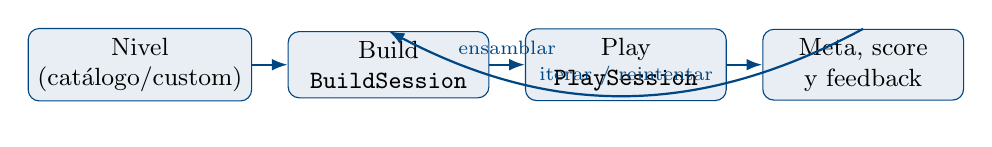
\begin{tikzpicture}[
    box/.style={draw=utecblue,rounded corners,fill=utecblue!9,
      minimum width=2.55cm,minimum height=0.8cm,align=center,font=\small},
    arrow/.style={-{Latex[length=2mm]},thick,utecblue}
  ]
    \node[box] (level) {Nivel\\(catálogo/custom)};
    \node[box,right=0.45cm of level] (build) {Build\\\texttt{BuildSession}};
    \node[box,right=0.45cm of build] (play) {Play\\\texttt{PlaySession}};
    \node[box,right=0.45cm of play] (result) {Meta, score\\y feedback};
    \draw[arrow] (level)--(build);
    \draw[arrow] (build)--node[above,font=\scriptsize]{ensamblar}(play);
    \draw[arrow] (play)--(result);
    \draw[arrow,bend left=28] (result.north) to node[above,font=\scriptsize]{iterar / reintentar} (build.north);
  \end{tikzpicture}
  \end{center}

  \vspace{0.15cm}
  \begin{itemize}
    \item \textbf{Build:} el jugador edita un \texttt{BuildModel} sobre \texttt{EditorGrid}; la sesión guarda selección, orientación y reposicionamiento.
    \item \textbf{Transición a Play:} \texttt{PlaySession} clona el modelo (\emph{runtime model}), crea el mundo físico/terreno y \texttt{PhysicsAssembler} materializa rigid bodies y joints.
    \item \textbf{Simulación:} cada frame actualiza activaciones, avanza la física, procesa impactos/eventos (roturas, eyecciones, consumo) y evalúa la meta.
    \item \textbf{Resultado:} se calcula el score del intento y el jugador puede volver a construcción para mejorar el diseño.
  \end{itemize}
\end{frame}

\begin{frame}{Condición de victoria: ventana de meta}
  \begin{columns}[T]
    \column{0.5\textwidth}
    \begin{block}{\texttt{GoalWindowTracker}}
      \begin{itemize}
        \item La ventana inicia cuando el \emph{Conductor} entra/toca el área de meta (considerando cruce entre frames).
        \item Una vez iniciada, la ventana no se cancela si el Conductor sale.
        \item Se registran partes iniciales y pasajeros entregados según las reglas del objetivo.
        \item La victoria se completa tras sostener la condición por la ventana requerida ($\approx 3\,\mathrm{s}$).
      \end{itemize}
    \end{block}
    \column{0.46\textwidth}
    \begin{block}{Lectura de juego}
      No basta con ``rozar'' la meta: el diseño debe llegar y mantenerse funcional.
      \vspace{0.15cm}
      \begin{itemize}
        \item Roturas estructurales pueden impedir la entrega.
        \item Explosiones o impactos cambian el resultado.
        \item La ruta y el tiempo influyen en el score.
      \end{itemize}
    \end{block}
  \end{columns}
\end{frame}

\section{Construcción y contenido}

\begin{frame}{Construcción del vehículo: grilla y sesiones}
  \begin{columns}[T]
    \column{0.53\textwidth}
    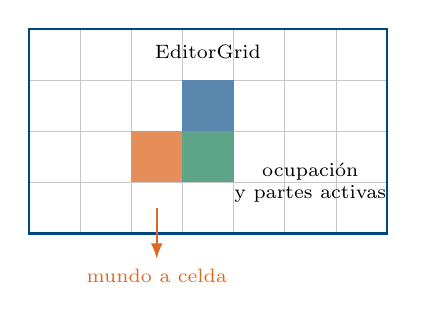
\begin{tikzpicture}[scale=0.65]
      \draw[step=1cm,gray!45,very thin] (0,0) grid (7,4);
      \draw[thick,utecblue] (0,0) rectangle (7,4);
      \fill[utecorange!75] (2,1) rectangle (3,2);
      \fill[utecgreen!70] (3,1) rectangle (4,2);
      \fill[utecblue!65] (3,2) rectangle (4,3);
      \draw[-{Latex[length=2mm]},thick,utecorange] (2.5,0.5)--(2.5,-0.5)
        node[below,font=\scriptsize] {mundo a celda};
      \node[font=\scriptsize] at (3.5,3.55) {EditorGrid};
      \node[font=\scriptsize,align=center] at (5.5,1.0)
        {ocupación\\y partes activas};
    \end{tikzpicture}
    \column{0.43\textwidth}
    \begin{block}{\texttt{EditorGrid} / \texttt{BuildSession}}
      \begin{itemize}
        \item Conversión mundo$\leftrightarrow$celda, límites y ocupación.
        \item Colocar, quitar, rotar, limpiar y desplazar contenidos.
        \item Selección, pickup y reposicionamiento desacoplados de la UI.
      \end{itemize}
    \end{block}
  \end{columns}

  \vspace{0.1cm}
  \begin{block}{Coordenadas discretas}
    \[
      \mathbf{c} = \left\lfloor
      \frac{\mathbf{p}_{world} - \mathbf{o}}{s}
      \right\rfloor,
      \qquad
      \mathbf{p}_{world} = \mathbf{o} + s\,\mathbf{c}, \quad s=\texttt{cellSize}.
    \]
  \end{block}
\end{frame}

\begin{frame}{Partes, conectores y reglas de build}
  \begin{columns}[T]
    \column{0.5\textwidth}
    \begin{block}{Modelo de partes}
      \begin{itemize}
        \item \texttt{Part}: celda, id, orientación, rol/contenido y cuerpo físico.
        \item \texttt{PartDefinition}: masa, forma, conectores, comportamiento y offsets.
        \item \texttt{BuildModel}: placements, conexiones y reglas de colocación.
      \end{itemize}
    \end{block}
    \column{0.46\textwidth}
    \begin{block}{Partes (nombres in-game)}
      \begin{itemize}
        \item \textbf{Cabina del chofer} (\emph{Driver Box}) y \textbf{Conductor} (contenido).
        \item \textbf{Cabina de pasajero} (\emph{Square Block}).
        \item \textbf{Llanta} (\emph{Wheel}), \textbf{Ventilador} (\emph{Fan}).
        \item \textbf{Inflador de globos} (\emph{Wind Sail}).
        \item \textbf{Tanque SOLGAS} (\emph{TNT}).
      \end{itemize}
    \end{block}
  \end{columns}

  \vspace{0.1cm}
  \begin{itemize}
    \item El Conductor no se coloca suelto: va dentro de la Cabina del chofer (una por build).
    \item Las conexiones válidas dependen de compatibilidad y máscaras de conectores; piezas acoplables pueden auto-orientarse al construir.
    \item Inercia de caja homogénea (aprox. para rigid body rectangular): \(
      I = \frac{1}{12}m(w^2+h^2).
    \)
  \end{itemize}
\end{frame}

\begin{frame}{Editor de niveles (contenido custom)}
  \begin{columns}[T]
    \column{0.52\textwidth}
    \begin{block}{\texttt{CustomLevelEditorScene}}
      Herramientas de authoring observadas:
      \begin{itemize}
        \item \textbf{Terrain}: editar geometría del terreno.
        \item \textbf{Grid}: definir zona/soporte de construcción.
        \item \textbf{Goal}: ubicar el área objetivo.
        \item \textbf{Passenger}: colocar pasajeros del nivel.
        \item \textbf{Eraser}: borrar elementos del diseño.
      \end{itemize}
    \end{block}
    \column{0.44\textwidth}
    \begin{block}{Datos y alcance}
      \begin{itemize}
        \item Persistencia/catálogo: \texttt{CustomLevelCatalog}, \texttt{CustomLevelData}.
        \item Configuración adicional del nivel (p. ej. selección de música).
        \item Define el reto/escenario; es distinto del editor de vehículo.
        \item El nivel custom se juega con el mismo pipeline build $\rightarrow$ play $\rightarrow$ score.
      \end{itemize}
    \end{block}
  \end{columns}
\end{frame}

\section{Puntuación y ranking}

\begin{frame}{Cómo se consiguen puntos y cómo se rankea}
  \begin{columns}[T]
    \column{0.5\textwidth}
    \begin{block}{Puntaje (alto nivel, \texttt{score-v2})}
      \begin{itemize}
        \item \textbf{Pickup/delivery de pasajeros:} recompensan rescatar y entregar.
        \item \textbf{Entrega de partes:} premia conservar/entregar el vehículo inicial.
        \item \textbf{Velocidad:} bono por completar rápido (acotado por tiempo límite).
        \item \textbf{Construction penalty:} usar muchas piezas extra reduce el total efectivo (incentiva eficiencia).
        \item \textbf{Validez:} intentos con estadísticas inconsistentes no puntúan como válidos.
      \end{itemize}
    \end{block}
    \column{0.46\textwidth}
    \begin{block}{Ranking}
      \begin{itemize}
        \item Se registra el intento (\texttt{RunStatistics}, breakdown, \texttt{RunCapture}).
        \item El ranking prioriza el \textbf{total} de score.
        \item En empates se usan criterios secundarios (p. ej. menor tiempo del Conductor en el flujo de leaderboard).
        \item Existe comparación local/reglas y envío/consulta remota de leaderboard cuando aplica.
      \end{itemize}
    \end{block}
  \end{columns}

  \vspace{0.1cm}
  \begin{center}
    \small \textit{acciones del run} $\rightarrow$ \textit{breakdown} $\rightarrow$ \textit{total} $\rightarrow$ \textit{posición}.
  \end{center}
\end{frame}

\section{Motor de física y pipeline}

\begin{frame}{Del build a la simulación (rigid bodies)}
  \begin{center}
  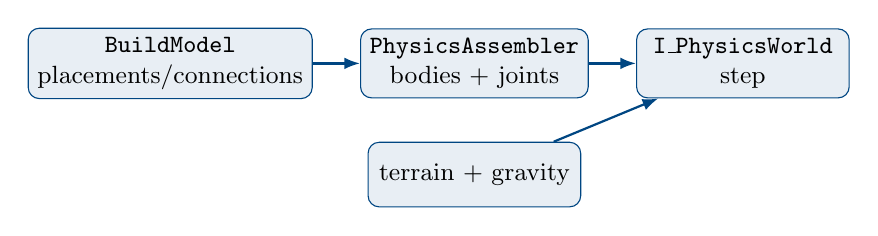
\begin{tikzpicture}[
    box/.style={draw=utecblue,rounded corners,fill=utecblue!9,
      minimum width=2.7cm,minimum height=0.82cm,align=center,font=\small},
    arrow/.style={-{Latex[length=2mm]},thick,utecblue}
  ]
    \node[box] (placements) {\texttt{BuildModel}\\placements/connections};
    \node[box,right=0.6cm of placements] (assembly) {\texttt{PhysicsAssembler}\\bodies + joints};
    \node[box,right=0.6cm of assembly] (world) {\texttt{I\_PhysicsWorld}\\step};
    \node[box,below=0.55cm of assembly] (terrain) {terrain + gravity};
    \draw[arrow] (placements)--(assembly);
    \draw[arrow] (assembly)--(world);
    \draw[arrow] (terrain)--(world);
  \end{tikzpicture}
  \end{center}

  \begin{block}{Motor custom}
    Evolución de Box2D a un motor propio de rigid bodies e impulsos:
    \texttt{World}, \texttt{RigidBody}, \texttt{Joint}, pipeline de step
    (broad/narrow, velocity, position, cleanup) y análisis estructural.
  \end{block}
\end{frame}

\begin{frame}{Paso de simulación: integración y solver iterativo}
  \begin{block}{Integración (semi-implícita, por substep)}
    Para cada cuerpo dinámico con masa $m$ e inversa $m^{-1}$:
    \[
      \mathbf{v} \leftarrow \mathbf{v} + \Delta t\left(\mathbf{g} + m^{-1}\mathbf{F}_{ext}\right),
      \qquad
      \mathbf{x} \leftarrow \mathbf{x} + \Delta t\,\mathbf{v},
      \qquad
      \theta \leftarrow \theta + \Delta t\,\omega.
    \]
    (Con damping aplicado en el step para estabilidad numérica.)
  \end{block}

  \vspace{0.05cm}
  \begin{block}{Resolución de constraints por iteraciones}
    En cada substep:
    \[
      \underbrace{\text{integrate}}_{\mathbf{v},\mathbf{x},\theta}
      \rightarrow \text{broad/narrow}
      \rightarrow \underbrace{\text{velocity solver}}_{\text{impulses}}
      \rightarrow \underbrace{\text{position correction}}_{\text{drift/penetration}}.
    \]
    Esto aproxima la solución global resolviendo contactos y joints repetidamente.
  \end{block}
\end{frame}

\begin{frame}{Velocity constraints: joints y contactos}
  \begin{block}{Revolute joint (anclajes coincidentes)}
    Error de velocidad relativa en el ancla $\mathbf{r}$:
    \[
      \mathbf{v}_{rel} = (\mathbf{v}_B + \boldsymbol{\omega}_B \times \mathbf{r}_B) -
      (\mathbf{v}_A + \boldsymbol{\omega}_A \times \mathbf{r}_A), \qquad
      \mathbf{C} = \mathbf{p}_B - \mathbf{p}_A.
    \]
    Impulso lineal con \emph{Baumgarte bias}:
    \[
      \boldsymbol{\lambda} = -\mathbf{K}^{-1}\left(\mathbf{v}_{rel} + \frac{\beta}{\Delta t}\mathbf{C}\right),
      \qquad
      \Delta\mathbf{v} = \pm m^{-1}\boldsymbol{\lambda},\;
      \Delta\omega = \pm I^{-1}(\mathbf{r}\times\boldsymbol{\lambda}).
    \]
  \end{block}

  \begin{block}{Weld joint y contacto}
    \textbf{Weld}: añade constraint angular
    \(
      C_\theta = (\theta_B-\theta_A)-\theta_{ref},\;
      \lambda_\theta \approx -\frac{\omega_{rel} + \frac{\beta}{\Delta t}C_\theta}{I_A^{-1}+I_B^{-1}}
    \).
    \textbf{Contacto}: impulso normal (no-penetración/restitución) y fricción tangencial acotada
    \( |j_t| \le \mu j_n \), con acumulación/clamping por punto de contacto.
  \end{block}
\end{frame}

\begin{frame}{Position correction (estabilización)}
  \begin{columns}[T]
    \column{0.5\textwidth}
    \begin{block}{Corrección posicional de joints}
      Para reducir drift de anclajes:
      \[
        \Delta \mathbf{p} \propto -\beta\,\mathbf{K}^{-1}\mathbf{C}, \qquad
        \mathbf{C}=\mathbf{p}_B-\mathbf{p}_A.
      \]
      \textbf{Weld joint}: además corrige error angular
      \(
        C_\theta = \operatorname{wrap}((\theta_B-\theta_A)-\theta_{ref})
      \)
      distribuyendo rotación según inercias inversas.
    \end{block}
    \column{0.46\textwidth}
    \begin{block}{Contactos y estabilidad}
      \begin{itemize}
        \item Proyección/corrección para resolver penetraciones residuales tras el velocity solve.
        \item Actualización de AABB tras mover cuerpos.
        \item Iteraciones de posición mejoran stacking y rigidez aparente sin volver el solver global.
      \end{itemize}
      \vspace{0.1cm}
      \small (El detalle numérico exacto depende del caso de colisión/manifold, pero el objetivo es el mismo: consistencia geométrica estable.)
    \end{block}
  \end{columns}
\end{frame}

\section{Colisiones y respuesta}

\begin{frame}{Broad/Narrow phase y manifold}
  \begin{columns}[T]
    \column{0.5\textwidth}
    \begin{block}{Broad phase (AABB)}
      Descarte por solapamiento de intervalos:
      \[
        [x_{min}^A,x_{max}^A]\cap[x_{min}^B,x_{max}^B]\neq\varnothing,\;
        [y_{min}^A,y_{max}^A]\cap[y_{min}^B,y_{max}^B]\neq\varnothing.
      \]
      Suficiente para la escala actual; estructuras como BVH/grid quedan como optimización futura.
    \end{block}
    \column{0.46\textwidth}
    \begin{block}{Narrow phase (SAT / dispatch)}
      \begin{itemize}
        \item SAT para convexos: eje separador o solapamiento mínimo $\Rightarrow (\mathbf{n},\delta)$.
        \item Rutinas especializadas por par de formas.
        \item Manifold con uno o más puntos: $\mathbf{p},\mathbf{n},\delta$ e impulsos acumulados (warm starting).
      \end{itemize}
    \end{block}
  \end{columns}
\end{frame}

\begin{frame}{Impulso de contacto: normal y fricción}
  \begin{block}{Velocidad relativa y masa efectiva}
    \[
      \mathbf{v}_{rel}=(\mathbf{v}_B+\omega_B\mathbf{r}_B^\perp)-(\mathbf{v}_A+\omega_A\mathbf{r}_A^\perp), \qquad
      m_{eff,n}^{-1}=m_A^{-1}+m_B^{-1}+\frac{(\mathbf{r}_A\times\mathbf{n})^2}{I_A}+\frac{(\mathbf{r}_B\times\mathbf{n})^2}{I_B}.
    \]
  \end{block}

  \begin{columns}[T]
    \column{0.5\textwidth}
    \begin{block}{Normal (restitución)}
      \[
        j_n = \frac{-(1+e)\,\min(\mathbf{v}_{rel}\cdot\mathbf{n},0)}{m_{eff,n}^{-1}}, \qquad j_n \ge 0.
      \]
      (La restitución se aplica en impactos significativos; el impulso se acumula/clampa.)
    \end{block}
    \column{0.46\textwidth}
    \begin{block}{Fricción de Coulomb}
      \[
        j_t = \frac{-(\mathbf{v}_{rel}\cdot\mathbf{t})}{m_{eff,t}^{-1}}, \qquad |j_t| \le \mu j_n.
      \]
      Con $\mathbf{t}\perp\mathbf{n}$ y acumulación para estabilidad de contacto.
    \end{block}
  \end{columns}
\end{frame}

\section{Activaciones y eventos importantes}

\begin{frame}{Activaciones: fuerzas, impulsos y eventos}
  \begin{columns}[T]
    \column{0.33\textwidth}
    \begin{block}{Ventilador (\emph{Fan})}
      \begin{itemize}
        \item Propulsión persistente mientras está activo.
        \item Aplica \textbf{fuerza continua} al cuerpo (aceleración dependiente de $m$): $\Delta\mathbf{v}\approx \Delta t\,\mathbf{F}/m$.
      \end{itemize}
    \end{block}
    \column{0.33\textwidth}
    \begin{block}{Inflador de globos (\emph{Wind Sail})}
      \begin{itemize}
        \item Propulsión direccional activable por el jugador.
        \item Modelada como \textbf{fuerza aplicada} durante su estado activo (no un impulso instantáneo único).
      \end{itemize}
    \end{block}
    \column{0.33\textwidth}
    \begin{block}{Tanque SOLGAS (\emph{TNT})}
      \begin{itemize}
        \item Evento explosivo: impulso radial atenuado por distancia.
        \item Puede afectar cuerpos/joints cercanos, activar cadenas y remover la pieza tras detonación.
        \item Impactos fuertes y contexto (contenedor/contenido) alteran el resultado.
      \end{itemize}
    \end{block}
  \end{columns}

  \vspace{0.1cm}
  \begin{alertblock}{Foco}
    Se prioriza modelar correctamente la diferencia \emph{fuerza sostenida} vs \emph{impulso/evento discreto}; detalles de timers secundarios no son centrales para la física del sistema.
  \end{alertblock}
\end{frame}

\section{Joints y estrés estructural}

\begin{frame}{Ensamblado de joints: revolute y weld}
  \begin{columns}[T]
    \column{0.5\textwidth}
    \begin{block}{\texttt{revolute joint}}
      Restringe traslación relativa en el ancla (2 DoF lineales):
      \[
        \mathbf{C}_{lin} = \mathbf{p}_B - \mathbf{p}_A = \mathbf{0},
      \]
      permitiendo rotación relativa.
    \end{block}
    \column{0.46\textwidth}
    \begin{block}{\texttt{weld joint}}
      Añade restricción angular (rigidez):
      \[
        C_{ang} = (\theta_B - \theta_A) - \theta_{ref} = 0.
      \]
      Útil para uniones rígidas del chasis/estructura.
    \end{block}
  \end{columns}

  \vspace{0.15cm}
  \begin{itemize}
    \item \texttt{BuildModel::GetConnections()} define pares/anclas; \texttt{PhysicsAssembler} crea los joints físicos.
    \item El solver usa impulsos iterativos + corrección posicional (Baumgarte) para mantener las constraints estables.
  \end{itemize}
\end{frame}

\begin{frame}{Sistema de grafo para estrés local}
  \begin{block}{Motivación}
    La rotura de un joint debe depender de la \textbf{carga local} que soporta según la topología del vehículo, no de una magnitud global uniforme.
  \end{block}

  \begin{itemize}
    \item \textbf{Rebuild por step:} \texttt{Structural::Graph} se reconstruye con cuerpos y joints activos.
    \item \textbf{Prueba de puente:} para evaluar un joint se excluye temporalmente y se exploran componentes conectados (BFS) desde cada cuerpo.
    \item \textbf{Componente dependiente:} si separa el grafo (\emph{bridge}), se selecciona el lado dependiente usando la gravedad (COM a lo largo de $\mathbf{g}$, con desempate por masa); si hay redundancia, la carga efectiva se atenúa.
    \item \textbf{Carga local:} masa dependiente, \emph{lever arm} $\mathbf{r}=\mathbf{COM}_{dep}-\mathbf{anchor}$, redundancia y factores de damping (masa, palanca, tipo de joint).
  \end{itemize}
\end{frame}

\begin{frame}{Estrés local y criterio de rotura}
  \begin{block}{Acumulación y damping}
    Durante el velocity solve se registra un esfuerzo instantáneo por joint (derivado del impulso aplicado, $s_{inst}$) y se conserva el pico del step:
    \[
      s_{peak} \leftarrow \max(s_{peak}, s_{inst}), \qquad
      s_{local} = \frac{s_{peak}}{d_{mass}\, d_{lever}\, d_{joint}\, d_{red}}.
    \]
    Los factores $d_{\cdot}$ provienen de la carga topológica local (masa, brazo de palanca, redundancia, y ajuste para \texttt{revolute joint}).
  \end{block}

  \begin{block}{Rotura}
    \[
      \text{break if}\quad s_{local} \ge \tau \cdot R_{joint},
    \]
    donde $\tau$ es el umbral global y $R_{joint}$ la resistencia del joint (p. ej. configurable en \texttt{weld joint}).
    Joints rotos se limpian del mundo, generando cambios estructurales reales en la simulación.
  \end{block}
\end{frame}

\begin{frame}{Localidad del grafo vs sensibilidad global}
  \begin{columns}[T]
    \column{0.5\textwidth}
    \begin{block}{Con grafo (local)}
      \begin{itemize}
        \item Cada joint ``siente'' principalmente el subgrafo que depende de él.
        \item Bridges concentran carga; ciclos/redundancias la reparten.
        \item Diseños grandes pero bien soportados no fuerzan roturas irreales en joints alejados.
        \item Mejor sensación de integridad estructural por zona del vehículo.
      \end{itemize}
    \end{block}
    \column{0.46\textwidth}
    \begin{block}{Sin grafo (global/ingenuo)}
      \begin{itemize}
        \item Umbrales ligados a masa total o respuestas uniformes escalan mal con el tamaño.
        \item En vehículos grandes, impactos moderados pueden sobreatensionar joints no relacionados.
        \item Roturas en cadena poco plausibles y difícil \emph{tuning}.
        \item Se pierde la localidad: el mismo joint se vuelve más frágil solo por añadir masa distante.
      \end{itemize}
    \end{block}
  \end{columns}

  \vspace{0.1cm}
  \begin{center}
    \small El coste extra es análisis topológico acotado al tamaño del vehículo, apropiado para el alcance del juego.
  \end{center}
\end{frame}

\section{Detalles relevantes y cierre}

\begin{frame}{Otros aspectos técnicos y de producto destacables}
  \begin{itemize}
    \item \textbf{Eventos en runtime:} impactos, eyección de contenidos, consumo de Tanque SOLGAS, limpieza de joints rotos y protección breve en el primer aterrizaje para evitar fallos espurios.
    \item \textbf{Separación de responsabilidades:} modelo de build, ensamblado físico, simulación y render desacoplados (el render lee estado, no decide física).
    \item \textbf{Pipeline de step explícito:} integración $\rightarrow$ broad/narrow $\rightarrow$ velocity iterations $\rightarrow$ position iterations $\rightarrow$ cleanup.
    \item \textbf{Progresión completa:} además de física, el proyecto integra meta, scoring versionado, captura de intentos y soporte de leaderboard/ranking.
    \item \textbf{Contenido y rejugabilidad:} niveles de catálogo y editor de niveles custom amplían el espacio de diseño/prueba.
  \end{itemize}
\end{frame}

\begin{frame}{Conclusión}
  \begin{block}{Pipeline unificado}
    \[
      \text{diseño en grilla}
      \rightarrow \text{grafo de partes/conexiones}
      \rightarrow \text{rigid bodies + joints}
      \rightarrow \text{simulación + estrés local}
      \rightarrow \text{meta/score}.
    \]
  \end{block}

  \vspace{0.2cm}
  \begin{itemize}
    \item El juego combina authoring, iteración de diseño y física de rigid bodies con constraints.
    \item El grafo estructural aporta localidad y credibilidad a las roturas en vehículos complejos.
    \item Las fórmulas de integración, impulsos y corrección posicional sustentan la estabilidad observada en juego.
  \end{itemize}

  \vspace{0.25cm}
  \begin{center}
    \Large\textbf{¡Gracias! Preguntas}
  \end{center}
\end{frame}

\end{document}
